\RequirePackage{fix-cm}
\RequirePackage{amsmath} % there is a silly amsmath error that
                         % makes this necessary; comment
                         % usepackage amsmath whenever it occurs
                         % after documentclass -- Stefan 2016-01-19
%
%\documentclass{svjour3}                     % onecolumn (standard format)
%\documentclass[smallcondensed]{svjour3}     % onecolumn (ditto)
\documentclass[smallextended]{svjour3}       % onecolumn (second format)
%\documentclass[twocolumn]{svjour3}          % twocolumn
%
\smartqed  % flush right qed marks, e.g. at end of proof
%
% \usepackage{graphicx}
\usepackage{october}
% \usepackage{lineno}
% \newcommand{\plebeian}[0]{\textsc{anderson}}
% \newcommand{\aristocratic}[0]{\textsc{augustin}}
\newcommand{\anderson}[0]{\textit{Bool-A}}
\newcommand{\augustin}[0]{\textit{Bool-B}}
% For BJPS
% \hyphenpenalty=10000
% \hbadness=10000

%
% \usepackage{mathptmx}      % use Times fonts if available on your TeX system
%
% insert here the call for the packages your document requires
%\usepackage{latexsym}
% etc.
%
% please place your own definitions here and don't use \def but
% \newcommand{}{}
%
% Insert the name of "your journal" with
% \journalname{myjournal}
%

\begin{document}

\title{Asymmetry and the Geometry of Reason}
% \subtitle{Do you have a subtitle?\\ If so, write it here}

%\titlerunning{Short form of title}        % if too long for running head

\author{Anonymous}
% \author{Stefan Lukits}

%\authorrunning{Short form of author list} % if too long for running head

% \institute{Stefan Lukits \at
%               Department of Philosophy \\
%               1866 Main Mall \\
%               Buchanan E370 \\
%               Vancouver BC V6T 1Z1 \\
%               Canada \\
%               Tel.: +1-604-321-3440 \\
%               \email{sediomyle@gmail.com}
% }

\date{Received: date / Accepted: date}
% The correct dates will be entered by the editor

\maketitle

\begin{abstract}
  {\noindent}The geometry of reason is the view that the underlying
  topology for credence functions is a metric space, on the basis of
  which axioms and theorems of epistemic utility for partial beliefs
  are formulated. It implies that Jeffrey conditioning must cede to an
  alternative form of conditioning. The latter fails a long list of
  plausible expectations. One solution to this problem is to reject
  the geometry of reason and accept information theory in its stead.
  Information theory comes fully equipped with an axiomatic approach
  which covers probabilism, standard conditioning, and Jeffrey
  conditioning. It is not based on an underlying topology of a metric
  space, but uses a non-commutative divergence instead of a symmetric
  distance measure. I show that information theory, despite initial
  promise, also fails to accommodate basic epistemic intuitions.
\end{abstract}

\section{Introduction}
\label{intr}

Consider an idealized rational agent whose doxastic state at time $t$
can be characterized such that she entertains certain partial beliefs
with respect to a finite propositional algebra (the result of a die
roll, for example). At a later time $t'$ her beliefs may have changed
due to intervening evidence. The agent uses ampliative reasoning to
narrow down the set of logically coherent updates to a subset of
credences (a so-called credal state). In Bayesian epistemology, for
example, this credal state depends in some way on standard
conditioning, using conditional probabilities, if the rational agent
becomes certain of an event between $t$ and $t'$. It is sometimes
shown that based on a number of assumptions the updated partial
beliefs are in accordance with the probability axioms; or Bayes'
theorem; or Jeffrey conditioning; or the principle of minimum
cross-entropy.

James Joyce, in his paper \qeins{A Nonpragmatic Vindication of
  Probabilism,} uses a norm of gradational accuracy to identify
inadmissible partial beliefs, which are demonstrably inferior in
epistemic terms to those partial beliefs left in the updated credal
state. Demonstrable inferiority in Joyce is usually based on
supervaluationist semantics, when for example one credence is more
truth-defective than another credence in all possible worlds.

A set of partial beliefs can be genuinely defective in epistemic terms
compared to another set of partial beliefs if its truth estimates are
necessarily worse than the truth estimates of its rival. Note that
with an estimate, as opposed to a guess, I am not simply right or
wrong about the estimated quantity---I am instead more or less
accurate. This distinction is due to Richard Jeffrey (see
\scite{7}{jeffrey86}{}). Joyce uses his norm of gradational accuracy
together with six axioms (structure, extensionality, dominance,
normality, weak convexity, symmetry) to give an epistemic
justification of probabilism: the requirement for a rational agent to
keep her partial beliefs in keeping with the axioms of probability
theory.

It is a natural question to ask whether the same line of reasoning can
give us an epistemic justification of standard conditioning and
Jeffrey conditioning. The former updates partial beliefs in light of
an event that is known to be true based on intervening evidence, i.e.\
$P'(E)=1$ ($P'$ for the posterior, not necessarily a probability). The
latter updates partial beliefs in light of an event about which the
agent has shifted in uncertainty based on intervening evidence, i.e.\
$P'(E)=y$ where $y$ is not necessarily equal to $P(E)=x$, the prior of
$E$. In a series of articles that will be pivotal for the rest of this
paper, Hannes Leitgeb and Richard Pettigrew show that using Joyce's
approach, accuracy can be bifurcated into local and global accuracy.
For this bifurcation to give consistent results, the Brier score must
be used for Joyce's norm of gradational accuracy. The Brier score
vindicates standard conditioning and rules out Jeffrey conditioning. A
new type of conditioning, which I shall call LP conditioning, takes
the place of Jeffrey conditioning (for details see
\scite{7}{leitgebpettigrew10i}{}).

I will show that LP conditioning fails a host of expectations that are
reasonable to have for the kind of updating scenario that LP
conditioning addresses. Since Leitgeb and Pettigrew's reasoning is
valid, it cannot be sound. I identify a premise and call it the
geometry of reason, on which Leitgeb and Pettigrew unwittingly cast
doubt by reductio. The geometry of reason assumes that probability
distributions entertain a geometric relationship to each other. At
first, this assumption is natural: probability distributions can be
isomorphically identified with points in a simplex, which is a
well-behaved $(n-1)$-dimensional subset of $\mathbb{R}^{n}$ ($n$ is
the cardinality of the set of atoms belonging to the propositional
algebra---that the credences on this set determine the credences on
all propositions presumes probabilism). It seems natural to measure
the difference between probability distributions by imposing a
Euclidean metric on this space. Joyce uses this geometry of reason,
for example, by defining midpoints between credences ($0.5P+0.5Q$) and
requiring them to be epistemically symmetric with respect to their
parents $P$ and $Q$.

Leitgeb and Pettigrew muse about alternative geometries, especially
non-Euclidean ones. They suspect that these would be based on and in
the end reducible to Euclidean geometry but they do not entertain the
idea that they could drop the requirement of a metric topology
altogether (for the use of non-Euclidean geodesics in statistical
inference see \scite{7}{amari85}{}). Thomas Mormann explicitly warns
against the assumption that the metrics for a geometry of logic is
Euclidean by default: \qeins{All too often, we rely on geometric
  intuitions that are determined by Euclidean prejudices. The geometry
  of logic, however, does not fit the standard Euclidean metrical
  framework} (see \scite{8}{mormann05}{433}; also
\scite{7}{miller84}{}). Mormann concludes in his article
\qeins{Geometry of Logic and Truth Approximation,}

\begin{quotex}
  Logical structures come along with ready-made geometric structures
  that can be used for matters of truth approximation. Admittedly,
  these geometric structures differ from those we are accostumed [sic]
  with, namely, Euclidean ones. Hence, the geometry of logic is not
  Euclidean geometry. This result should not come as a big surprise.
  There is no reason to assume that the conceptual spaces we use for
  representing our theories and their relations have an [sic]
  Euclidean structure. On the contrary, this would appear to be an
  improbable coincidence. \scite{3}{mormann05}{453}
\end{quotex}

If the geometry of reason gives us bad results, we need to look for
alternatives. Joyce now appears to favour Bregman divergences
(personal communication) and an emphasis on scoring rules rather than
metrics (see \scite{7}{preddseiringer09}{}; for a connection between
proper scoring rules and Bregman divergences see
\scite{7}{abernethyfrongillo12}{}). Bregman divergences are a
generalization which encompasses Euclidean geometry (the squared
Euclidean distance is a Bregman divergence) and its alternatives (for
example the Kullback-Leibler divergence that I will mention below).
Joyce, in line with his use of supervaluationist semantics, considers
one credence epistemically inferior to another if it is inferior on
all Bregman divergences. If different divergences give different
results, inferiority cannot be established.

There is another way to relate probability distributions to each other
and formulate a concept of difference between them that is less
general than Bregman divergences. It is based on information theory,
originally conceived to model the extra coding required when the
sender gets the probability distribution of the alphabet not quite
right. There is a substantial formal theory of information,
serendipitously cast in terms of probabilities; there is a similarly
substantial formal theory of probabilities and Bayesian epistemology,
also cast in terms of probabilities. The formal theories are
different: one uses Shannon's entropy, a logarithmic measure of
difference; the other uses primarily ratios. It turns out that the
superficial differences are rooted in deep commonalities. Information
theory can serve as justification for Bayesian norms (probabilism,
standard conditioning, and Jeffrey conditioning, for the latter two
see \scite{8}{lukits15}{1697f}).

My claim is that this confluence of two formal theories has in itself
justificatory force. This justificatory force may be small, and there
are certainly detractors who claim that information theory sometimes,
if not often, gives the wrong results if applied to epistemology (see
\scite{7}{friedmanshimony71}{}; \scite{8}{diaconiszabell82}{829};
\scite{8}{skyrms87updating}{241}; \scite{8}{walley91}{266ff};
\scite{8}{wagner92}{255}; \scite{8}{howsonfranklin94}{465};
\scite{8}{uffink95}{14}; \scite{8}{mackay03}{308};
\scite{8}{gruenwaldhalpern03}{243ff}; \scite{8}{halpern03}{110};
\scite{8}{howsonurbach06}{287}; \scite{8}{neapolitanjiang14}{4012}). I
myself in this paper will add to the wrinkles that appear when
information theory and epistemology are wedded to each other. 

I will hopefully also show, however, that a Euclidean prejudice in
these matters is more deleterious. Joyce's supervaluationist solution
to these problems using Bregman divergences is certainly a reasonable
option. Yet just as there is something special about Euclidean
geometry and its attendant Brier scoring rule, there is something
special about information theory and its attendant Kullback-Leibler
divergence. My results in this paper are largely negative: there are
insurmountable problems for the geometry of reason; there are serious
problems for information theory. The positive aspect is that formal
accounts, when they sometimes show surprising coherence or when they
can be used to yield non-trivial theorems, supply epistemic
justification just in terms of their formal architecture. I hope to
contribute by adding to a sketch of one interesting formal
architecture, especially its description of how epistemology and
information theory interlock, and by identifying its problems.

\subsection{Expectations for Jeffrey-Type Updating Scenarios}
\label{subsec:vidiedoo}

For the remainder of this paper I will assume probabilism and an
isomorphism between probability distributions $P$ on an outcome space
$\Omega$ with $|\Omega|=n$ and points
$p\in\mathbb{S}^{n-1}\subset\mathbb{R}^{n}$ having coordinates
$p_{i}=P(\omega_{i}),i=1,\ldots,n$ and $\omega_{i}\in{}\Omega$. Since
the isomorphism is to a metric space, there is a concept of difference
between credence functions which can be used to formulate axioms
relating credences to epistemic utility and to justify or to criticize
contentious positions such as Bayesian conditionalization, the
principle of indifference, other forms of conditioning, or probabilism
itself (see \scite{7}{joyce98}{}; \scite{7}{leitgebpettigrew10ii}{};
and \scite{7}{greaveswallace06}{}).

For information theory, as opposed to the geometry of reason, the
underlying topology for credence functions is not a metric space (see
figures \ref{fig:contourslp} and \ref{fig:contoursrj} for
illustration). The term information geometry is due to Imre
Csisz{\'a}r, who considers the Kullback-Leibler divergence a
non-commutative (asymmetric) analogue of squared Euclidean distance
and derives several results that are intuitive information geometric
counterparts of standard results in Euclidean geometry (see chapter 3
of \scite{7}{csiszarshields04}{}).

Consider the following example of a Jeffrey-type updating scenario.

\begin{quotex}
  \beispiel{Sherlock Holmes}\label{ex:holmes} Sherlock Holmes
  attributes the following probabilities to the propositions $E_{i}$
  that $k_{i}$ is the culprit in a crime:
  $P(E_{1})=1/3,P(E_{2})=1/2,P(E_{3})=1/6$, where $k_{1}$ is Mr.\ R.,
  $k_{2}$ is Ms.\ S., and $k_{3}$ is Ms.\ T. Then Holmes finds some
  evidence which convinces him that $P'(F^{*})=1/2$, where $F^{*}$ is
  the proposition that the culprit is male and $P$ is relatively prior
  to $P'$. What should be Holmes' updated probability that Ms.\ S. is
  the culprit?
\end{quotex}

I will look at the recommendations of Jeffrey conditioning and LP
conditioning for {\xample} \ref{ex:holmes} in the next section. For
now note that LP conditioning violates all of the following plausible
expectations in \textbf{List A}\label{page:listone} for an amujus, an
\qnull{alternative method of updating for Jeffrey-type updating
  scenarios.} This is \textbf{List A}:

\begin{itemize}
\item \textsc{continuity} An amujus ought to be continuous with
  standard conditioning as a limiting case.
\item \textsc{regularity} An amujus ought not to assign a posterior
  probability of $0$ to an event which has a positive prior
  probability and about which the intervening evidence says nothing
  except that a strictly weaker event has a positive posterior
  probability.
\item \textsc{levinstein} An amujus ought not to give \qeins{extremely
    unattractive} results in a Levinstein scenario (see
  \scite{7}{levinstein12}{}, which not only articulates this failed
  expectation for LP conditioning, but also the previous two).
\item \textsc{invariance} An amujus ought to be partition invariant.
\item \textsc{expansibility} An amujus ought to be insensitive to an
  expansion of the event space by zero-probability events.
\item \textsc{horizon} An amujus ought to exhibit the horizon effect
  which makes probability distributions which are nearer to extreme
  probability distributions appear to be closer to each other than
  they really are.
\end{itemize}

Jeffrey conditioning and LP conditioning are both an amujus based on a
concept of quantitative difference between probability distributions.
Evidence appears in the form of a constraint on acceptable probability
distributions and the closest acceptable probability to the original
(relatively prior) probability distribution is chosen as its
successor. Here is \textbf{List B}\label{page:listtwo}, a list of
reasonable expectations one may have toward this concept of
quantitative difference (we call it a distance function for the
geometry of reason and a divergence for information theory). Let
$d(p,q)$ express this concept mathematically.

\begin{itemize}
\item \textsc{triangularity} The concept obeys the triangle
  inequality. If there is an intermediate probability distribution, it
  will not make the difference smaller: $d(p,r)\leq{}d(p,q)+d(q,r)$.
  Buying a pair of shoes is not going to be more expensive than buying
  the two shoes individually.
\item \textsc{collinear horizon} This expecation is just a more
  technical restatement of the \textsc{horizon} expectation in the
  previous list. If $p,p',q,q'$ are collinear with the centre of the
  simplex $m$ (whose coordinates are $m_{i}=1/n$ for all $i$) and an
  arbitrary but fixed boundary point $\xi\in\partial\mathbb{S}^{n-1}$
  and $p,p',q,q'$ are all between $m$ and $\xi$ with
  $\|p'-p\|=\|q'-q\|$ where $p$ is strictly closest to $m$, then
  $|d(p,p')|<|d(q,q')|$. For an illustration of this expectation see
  figure \ref{fig:conditions}. 
\item \textsc{transitivity of asymmetry} An ordered pair $(p,q)$ of
  simplex points associated with probability distributions is
  asymmetrically negative, positive, or balanced, so either
  $d(p,q)-d(q,p)<0$ or $d(p,q)-d(q,p)>0$ or $d(p,q)-d(q,p)=0$. If
  $(p,q)$ and $(q,r)$ are asymmetrically positive, $(p,r)$ ought not
  to be asymmetrically negative. Think of a bicycle route map with
  different locations at varying altitudes. If it takes 20 minutes to
  get from $A$ to $B$ but only 15 minutes to get from $B$ to $A$ then
  $(A,B)$ is asymmetrically positive. If $(A,B)$ and $(B,C)$ are
  asymmetrically positive, then $(A,C)$ ought not to be asymmetrically
  negative.
\end{itemize}

While the Kullback-Leibler divergence of information theory fulfills
all the expectations of \textbf{List A}, save \textsc{horizon}, it
fails all the expectations in \textbf{List B}. Conversely, the
Euclidean distance of the geometry of reason fulfills all the
expectations of \textbf{List B}, save \textsc{collinear horizon}, and
fails all the expectations in \textbf{List A}. Information theory has
its own axiomatic approach to justifying probabilism and standard
conditioning (see \scite{7}{shorejohnson80}{}). Information theory
also provides a justification for Jeffrey conditioning and generalizes
it (see \scite{7}{lukits15}{}). All of these virtues stand in contrast
to the violations of the expectations in \textbf{List B}. The rest of
this paper fills in the details of these violations both for the
geometry of reason and information theory, with the conclusion that
the case for the geometry of reason is hopeless while the case for
information theory is now a major challenge for future research
projects.

\section{Geometry of Reason versus Information Theory}
\label{grit}

Here is a simple example corresponding to example~\ref{ex:holmes}
where the distance of geometry and the divergence of information
theory differ. With this difference in mind, I will show how LP
conditioning fails the expectations outlined in \textbf{List A}.
Consider the following three points in three-dimensional space:

\begin{equation}
  \label{eq:e6}
    a=\left(\frac{1}{3},\frac{1}{2},\frac{1}{6}\right) \hspace{.5in}
    b=\left(\frac{1}{2},\frac{3}{8},\frac{1}{8}\right)  \hspace{.5in}
    c=\left(\frac{1}{2},\frac{5}{12},\frac{1}{12}\right)
\end{equation}

All three are elements of the simplex $\mathbb{S}^{2}$: their
coordinates add up to $1$. Thus they represent probability
distributions $A,B,C$ over a partition of the event space into three
mutually exclusive events. Now call $D_{\mbox{\tiny KL}}(B,A)$ the
Kullback-Leibler divergence of $B$ from $A$ defined as follows, where
$a_{i}$ are the Cartesian coordinates of $a$ (the base of the
logarithm is not important, in order to facilitate easy
differentiation I will use the natural logarithm):

\begin{equation}
  \label{eq:e7}
  D_{\mbox{\tiny KL}}(B,A)=\sum_{i=1}^{3}b_{i}\log\frac{b_{i}}{a_{i}}.
\end{equation}

Note that the Kullback-Leibler divergence, irrespective of dimension,
is always positive as a consequence of Gibbs' inequality (see
\scite{7}{mackay03}{}, sections 2.6 and 2.7).

The Euclidean distance is defined as follows:

\begin{equation}
  \label{eq:e3}
  \|B-A\|=\sqrt{\sum_{i=1}^{n}\left(b_{i}-a_{i}\right)^{2}}.
\end{equation}

The Euclidean distance $\|B-A\|$ is defined as in equation
(\ref{eq:e3}). What is remarkable about the three points in
(\ref{eq:e6}) is that

\begin{equation}
  \label{eq:e8}
  \|C-A\|\approx{}0.204<\|B-A\|\approx{}0.212
\end{equation}

and

\begin{equation}
  \label{eq:e9}
  D_{\mbox{\tiny KL}}(B,A)\approx{}0.0589<D_{\mbox{\tiny KL}}(C,A)\approx{}0.069.
\end{equation}

The Kullback-Leibler divergence and Euclidean distance give different
re\-commendations with respect to proximity. In terms of the global
inaccuracy measure presented in Leitgeb and Pettigrew (see
\scite{8}{leitgebpettigrew10i}{206}) and $E=W$ (all possible worlds
are epistemically accessible),

\begin{equation}
  \label{eq:e8a}
  \mbox{GExp}_{A}(C)\approx{}0.653<\mbox{GExp}_{A}(B)\approx{}0.656.
\end{equation}

Global inaccuracy reflects the Euclidean proximity relation, not the
re\-commendation of information theory. If $A$ corresponds to my prior
and my evidence is such that I must change the first coordinate to
$1/2$ (as in {\xample}~\ref{ex:holmes}) and nothing stronger, then
information theory via the Kullback-Leibler divergence re\-commends
the posterior corresponding to $B$; and the geometry of reason as
expounded in Leitgeb and Pettigrew recommends the posterior
corresponding to $C$. 

\subsection{LP conditioning and Jeffrey Conditioning}
\label{subsec:meexughi}

Here is a brief sketch how Leitgeb and Pettigrew arrive at posterior
probability distributions in Jeffrey-type updating scenarios. I will
call their method LP conditioning.

\begin{quotex}
  \beispiel{Abstract Holmes}\label{ex:abstract} Consider a possibility
  space $W=E_{1}\cup{}E_{2}\cup{}E_{3}$ (the $E_{i}$ are sets of
  states which are pairwise disjoint and whose union is $W$) and a
  partition $\mathcal{F}$ of $W$ such that
  $\mathcal{F}=\{F^{*},F^{**}\}=\{E_{1},E_{2}\cup{}E_{3}\}$.
\end{quotex}

Let $P$ be the prior probability function on $W$ and $P'$ the
posterior. I will keep the notation informal to make this simple, not
mathematically precise. Jeffrey-type updating scenarios give us new
information on the posterior probabilities of partitions such as
$\mathcal{F}$. In {\xample} \ref{ex:abstract}, let

\begin{equation}
  \label{eq:priors}
  \begin{array}{rcl}
    P(E_{1})&=&1/3 \\
    P(E_{2})&=&1/2 \\
    P(E_{3})&=&1/6
  \end{array}
\end{equation}

and the new evidence constrain $P'$ such that
$P'(F^{*})=1/2=P'(F^{**})$.

Jeffrey conditioning works on the following intuition, which elsewhere
I have called Jeffrey's updating principle \textsc{jup} (see also
\scite{7}{wagner02}{}). The posterior probabilities conditional on the
partition elements equal the prior probabilities conditional on the
partition elements since we have no information in the evidence that
they should have changed. Hence,

\begin{align}
  \label{eq:jc}
  &P'_{\mbox{\tiny JC}}(E_{i})&=&P'(E_{i}|F^{*})P'(F^{*})+P'(E_{i}|F^{**})P'(F^{**})\notag \\
  &&=&P(E_{i}|F^{*})P'(F^{*})+P(E_{i}|F^{**})P'(F^{**})
\end{align}

Jeffrey conditioning is controversial (for an introduction to Jeffrey
conditioning see \scite{7}{jeffrey65}{}; for its statistical and
formal properties see \scite{7}{diaconiszabell82}{}; for a pragmatic
vindication of Jeffrey conditioning see \scite{7}{armendt80}{}, and
\scite{7}{skyrms86}{}; for criticism see
\scite{7}{howsonfranklin94}{}). Information theory, however, supports
Jeffrey conditioning. Leitgeb and Pettigrew show that Jeffrey
conditioning does not in general pick out the minimally inaccurate
posterior probability distribution. If the geometry of reason as
presented in Leitgeb and Pettigrew is sound, this would constitute a
powerful criticism of Jeffrey conditioning. Leitgeb and Pettigrew
introduce an alternative to Jeffrey conditioning, which I call LP
conditioning. It proceeds as follows for {\xample} \ref{ex:abstract}
and in general provides the minimally inaccurate posterior probability
distribution in Jeffrey-type updating scenarios.

Solve the following two equations for $x$ and $y$:

\begin{equation}
  \label{eq:lpce}
  \begin{array}{rcl}
    P(E_{1})+x&=&P'(F^{*}) \\
    P(E_{2})+y+P(E_{3})+y&=&P'(F^{**})
  \end{array}
\end{equation}

and then set

\begin{equation}
  \label{eq:lpcf}
  \begin{array}{rcl}
    P'_{\mbox{\tiny LP}}(E_{1})&=&P(E_{1})+x \\
    P'_{\mbox{\tiny LP}}(E_{2})&=&P(E_{2})+y \\
    P'_{\mbox{\tiny LP}}(E_{3})&=&P(E_{3})+y
  \end{array}
\end{equation}

For the more formal and more general account see
\scite{8}{leitgebpettigrew10ii}{254}. The results for {\xample}
\ref{ex:abstract} are:

\begin{equation}
  \label{eq:lpcres}
  \begin{array}{rcl}
    P'_{\mbox{\tiny LP}}(E_{1})&=&1/2 \\
    P'_{\mbox{\tiny LP}}(E_{2})&=&5/12 \\
    P'_{\mbox{\tiny LP}}(E_{3})&=&1/12
  \end{array}
\end{equation}

Compare these results to the results of Jeffrey conditioning:

\begin{equation}
  \label{eq:jcres}
  \begin{array}{rcl}
    P'_{\mbox{\tiny JC}}(E_{1})&=&1/2 \\
    P'_{\mbox{\tiny JC}}(E_{2})&=&3/8 \\
    P'_{\mbox{\tiny JC}}(E_{3})&=&1/8
  \end{array}
\end{equation}

Note that (\ref{eq:priors}), (\ref{eq:jcres}), and (\ref{eq:lpcres})
correspond to $A,B,C$ in (\ref{eq:e6}). 

\section{Expectations for the Geometry of Reason}
\label{fivex}

This section provides more detail for the expectations in \textbf{List
  A} and shows how LP conditioning violates them.

\subsection{Continuity}
\label{Continuity}

LP conditioning violates \textsc{continuity} because standard
conditioning gives a different recommendation than a parallel sequence
of Jeffrey-type updating scenarios which get arbitrarily close to
standard event observation. This is especially troubling considering
how important the case for standard conditioning is to Leitgeb and
Pettigrew.

To illustrate a \textsc{continuity} violation, consider the case where
Sherlock Holmes reduces his credence that the culprit was male to
$\varepsilon_{n}=1/n$ for $n=4,5,\ldots$. The sequence
$\varepsilon_{n}$ is not meant to reflect a case where Sherlock Holmes
becomes successively more certain that the culprit was female. It is
meant to reflect countably many parallel scenarios which only differ
by the degree to which Sherlock Holmes is sure that the culprit was
female. These parallel scenarios give rise to a parallel sequence (as
opposed to a successive sequence) of updated probabilities
$P'_{\mbox{\tiny LP}}(F^{**})$ and another sequence of updated
probabilities $P'_{\mbox{\tiny JC}}(F^{**})$ ($F^{**}$ is the
proposition that the culprit is female). As $n\rightarrow\infty$, both
of these sequences go to one.

Straightforward conditionalization on the evidence that \qnull{the
  culprit is female} gives us 

\begin{equation}
  \label{eq:sherlockcontsc}
  \begin{array}{rcl}
  P'_{\mbox{\tiny SC}}(E_{1})&=&0\\
  P'_{\mbox{\tiny SC}}(E_{2})&=&3/4\\
  P'_{\mbox{\tiny SC}}(E_{3})&=&1/4.
\end{array}
\end{equation}

Letting $n\rightarrow\infty$ for Jeffrey conditioning yields

\begin{equation}
  \label{eq:sherlockcontjc}
  \begin{array}{rcccl}
  P'_{\mbox{\tiny JC}}(E_{1})&=&1/n&\rightarrow&0\\
  P'_{\mbox{\tiny JC}}(E_{2})&=&3(n-1)/4n&\rightarrow&3/4\\
  P'_{\mbox{\tiny JC}}(E_{3})&=&(n-1)/4n&\rightarrow&1/4,
\end{array}
\end{equation}

whereas letting $n\rightarrow\infty$ for LP conditioning yields

\begin{equation}
  \label{eq:sherlockcontlp}
  \begin{array}{rcccl}
  P'_{\mbox{\tiny LP}}(E_{1})&=&1/n&\rightarrow&0\\
  % this is mine, further down is Paul's 
  % P'_{\mbox{\tiny LP}}(E_{2})&=&(4n-1)/6n&\rightarrow&2/3\\
  % P'_{\mbox{\tiny LP}}(E_{3})&=&(2n-1)/6n&\rightarrow&1/3.
  P'_{\mbox{\tiny LP}}(E_{2})&=&(4n-3)/6n&\rightarrow&2/3\\
  P'_{\mbox{\tiny LP}}(E_{3})&=&(2n-5)/6n&\rightarrow&1/3.
\end{array}
\end{equation}

LP conditioning violates \textsc{continuity}.

\subsection{Regularity}
\label{Regularity}

LP conditioning violates \textsc{regularity} because formerly positive
probabilities can be reduced to $0$ even though the new information in
the Jeffrey-type updating scenario makes no such requirements (as is
usually the case for standard conditioning). Ironically, Jeffrey-type
updating scenarios are meant to be a better reflection of real-life
updating because they avoid extreme probabilities. 

The violation becomes serious if we are already sympathetic to an
infor\-ma\-tion-based account: the amount of information required to turn
a non-extreme probability into one that is extreme ($0$ or $1$) is
infinite. Whereas the geometry of reason considers extreme
probabilities to be easily accessible by non-extreme probabilities
under new information (much like a marble rolling off a table or a
bowling ball heading for the gutter), information theory envisions
extreme probabilities more like an event horizon. The nearer you are
to the extreme probabilities, the more information you need to move
on. For an observer, the horizon is never reached.

\begin{quotex}
  \beispiel{Regularity Holmes}\label{ex:regularity} Everything is as
  in {\xample} \ref{ex:holmes}, except that Sherlock Holmes becomes
  confident to a degree of $2/3$ that Mr.\ R is the culprit and
  updates his relatively prior probability distribution in
  (\ref{eq:priors}).
\end{quotex}

Then his posterior probabilities look as follows:

\begin{equation}
  \label{eq:sherlockposteriorjcreg}
  \begin{array}{rcl}
  P'_{\mbox{\tiny JC}}(E_{1})&=&2/3\\
  P'_{\mbox{\tiny JC}}(E_{2})&=&1/4\\
  P'_{\mbox{\tiny JC}}(E_{3})&=&1/12
\end{array}
\end{equation}

\begin{equation}
  \label{eq:sherlockposteriorlpreg}
  \begin{array}{rcl}
  P'_{\mbox{\tiny LP}}(E_{1})&=&2/3\\
  P'_{\mbox{\tiny LP}}(E_{2})&=&1/3\\
  P'_{\mbox{\tiny LP}}(E_{3})&=&0
\end{array}
\end{equation}

With LP conditioning, Sherlock Holmes' subjective probability that
Ms.\ T is the culprit in {\xample} \ref{ex:regularity} has been reduced
to zero. No finite amount of information could bring Ms.\ T back into
consideration as a culprit in this crime, and Sherlock Holmes should
be willing to bet any amount of money against a penny that she is not
the culprit---even though his evidence is nothing more than an
increase in the probability that Mr.\ R is the culprit.

LP conditioning violates \textsc{regularity}.

\subsection{Levinstein}
\label{Levinstein}

LP conditioning violates \textsc{levinstein} because of \qeins{the
  potentially dramatic effect [LP conditioning] can have on the
  likelihood ratios between different propositions}
\scite{3}{levinstein12}{419}. Consider Benjamin Levinstein's example:

\begin{quotex}
  \beispiel{Levinstein's Ghost}\label{ex:levinstein} There is a car
  behind an opaque door, which you are almost sure is blue but which
  you know might be red. You are almost certain of materialism, but
  you admit that there's some minute possibility that ghosts exist.
  Now the opaque door is opened, and the lighting is fairly good. You
  are quite surprised at your sensory input: your new credence that
  the car is red is very high.
\end{quotex}

Jeffrey conditioning leads to no change in opinion about ghosts. Under
LP conditioning, however, seeing the car raises the probability that
there are ghosts to an astonishing 47\%, given Levinstein's reasonable
priors. Levinstein proposes a logarithmic inaccuracy measure as a
remedy to avoid violation of \textsc{levinstein}. As a special case of
applying a Levinstein-type logarithmic inaccuracy measure, information
theory does not violate \textsc{levinstein}.

\subsection{Invariance}
\label{Invariance}

LP conditioning violates \textsc{invariance} because two agents who
have identical credences with respect to a partition of the event
space may disagree about this partition after LP conditioning, even
when the Jeffrey-type updating scenario provides no new information
about the more finely grained partitions on which the two agents
disagree. 

\begin{quotex}
  \beispiel{Jane Marple}\label{ex:marple} Jane Marple is on the same
  case as Sherlock Holmes in {\xample} \ref{ex:holmes} and arrives at
  the same relatively prior probability distribution as Sherlock
  Holmes (I will call Jane Marple's relatively prior probability
  distribution $Q$ and her posterior probability distribution $Q'$).
  Jane Marple, however, has a more finely grained probability
  assignment than Sherlock Holmes and distinguishes between the case
  where Ms.\ S went to boarding school with her, of which she has a
  vague memory, and the case where Ms.\ S did not and the vague memory
  is only about a fleeting resemblance of Ms.\ S with another boarding
  school mate. Whether or not Ms.\ S went to boarding school with Jane
  Marple is completely beside the point with respect to the crime, and
  Jane Marple considers the possibilities equiprobable whether or not
  Ms.\ S went to boarding school with her.
\end{quotex}

Let $E_{2}\equiv{}E_{2}^{*}\vee{}E_{2}^{**}$, where $E_{2}^{*}$ is the
proposition that Ms.\ S is the culprit and she went to boarding school
with Jane Marple and $E_{2}^{**}$ is the proposition that Ms.\ S is
the culprit and she did not go to boarding school with Jane Marple.
Then

\begin{equation}
  \label{eq:marpleprior}
  \begin{array}{rcl}
  Q(E_{1})&=&1/3\\
  Q(E_{2}^{*})&=&1/4\\
  Q(E_{2}^{**})&=&1/4\\
  Q(E_{3})&=&1/6.
\end{array}
\end{equation}

Now note that while Sherlock Holmes and Jane Marple agree on the
relevant facts of the criminal case (who is the culprit?) in their
posterior probabilities if they use Jeffrey conditioning,

\begin{equation}
  \label{eq:sherlockposteriorjc}
  \begin{array}{rcl}
  P'_{\mbox{\tiny JC}}(E_{1})&=&1/2\\
  P'_{\mbox{\tiny JC}}(E_{2})&=&3/8\\
  P'_{\mbox{\tiny JC}}(E_{3})&=&1/8
\end{array}
\end{equation}

\begin{equation}
  \label{eq:marpleposteriorjc}
  \begin{array}{rcl}
  Q'_{\mbox{\tiny JC}}(E_{1})&=&1/2\\
  Q'_{\mbox{\tiny JC}}(E_{2}^{*})&=&3/16\\
  Q'_{\mbox{\tiny JC}}(E_{2}^{**})&=&3/16\\
  Q'_{\mbox{\tiny JC}}(E_{3})&=&1/8
\end{array}
\end{equation}

they do not agree if they use LP conditioning,

\begin{equation}
  \label{eq:sherlockposteriorlp}
  \begin{array}{rcl}
  P'_{\mbox{\tiny LP}}(E_{1})&=&1/2\\
  P'_{\mbox{\tiny LP}}(E_{2})&=&5/12\\
  P'_{\mbox{\tiny LP}}(E_{3})&=&1/12
\end{array}
\end{equation}

\begin{equation}
  \label{eq:marpleposteriorlp}
  \begin{array}{rcl}
  Q'_{\mbox{\tiny LP}}(E_{1})&=&1/2\\
  Q'_{\mbox{\tiny LP}}(E_{2}^{*})&=&7/36\\
  Q'_{\mbox{\tiny LP}}(E_{2}^{**})&=&7/36\\
  Q'_{\mbox{\tiny LP}}(E_{3})&=&1/9.
\end{array}
\end{equation}

LP conditioning violates \textsc{invariance}.

\subsection{Expansibility}
\label{Expansibility}

One particular problem with the lack of invariance for LP conditioning
is how zero-probability events should be included in the list of prior
probabilities that determines the value of the posterior
probabilities. Consider

\begin{equation}
  \label{eq:reginvone}
  \begin{array}{rcl}
  P(X_{1})&=&0\\
  P(X_{2})&=&0.3\\
  P(X_{3})&=&0.6\\
  P(X_{4})&=&0.1\\
\end{array}
\end{equation}

That $P(X_{1})=0$ may be a consequence of standard conditioning in a
previous step. Now the agent learns that $P'(X_{3}\vee{}X_{4})=0.5$.
Should the agent update on the list presented in (\ref{eq:reginvone})
or on the following list:

\begin{equation}
  \label{eq:reginvtwo}
  \begin{array}{rcl}
  P(X_{2})&=&0.3\\
  P(X_{3})&=&0.6\\
  P(X_{4})&=&0.1\\
\end{array}
\end{equation}

Whether you update on (\ref{eq:reginvone}) or (\ref{eq:reginvtwo})
makes no difference to Jeffrey conditioning, but due to the lack of
invariance it makes a difference to LP conditioning, so the geometry
of reason needs to find a principled way to specify the appropriate
prior probabilities. The only non-arbitrary way to do this is either
to include or to exclude all zero probability events on the list. This
strategy, however, sounds ill-advised unless one signs on to a
stronger version of \textsc{regularity} and requires that only a fixed
set of events can have zero probabilities (such as logical
contradictions), but then the geometry of reason ends up in the
catch-22 of LP conditioning running afoul of \textsc{regularity}.

LP conditioning violates \textsc{expansibility}.

\subsection{Horizon}
\label{Horizon}

\begin{quotex}
  \beispiel{Undergraduate Complaint}\label{ex:complaint} An
  undergraduate student complains to the department head that the
  professor will not reconsider an 89\% grade (which misses an A+ by
  one percent) when reconsideration was given to other students with a
  67\% grade (which misses a B- by one percent).
\end{quotex}

Intuitions may diverge, but the professor's reasoning is as follows.
To improve a 60\% paper by ten percent is easily accomplished: having
your roommate check your grammar, your spelling, and your line of
argument will sometimes do the trick. It is incomparably more
difficult to improve an 85\% paper by ten percent: it may take doing a
PhD to turn a student who writes the former into a student who writes
the latter. A maiore ad minus, the step from 89\% to 90\% is greater
than the step from 67\% to 68\%.

Another example for the horizon effect is George Schlesinger's
comparison between the risk of a commercial airplane crash and the
risk of a military glider landing in enemy territory.

\begin{quotex}
  \beispiel{Airplane Gliders}\label{ex:schlesinger} Compare two
  scenarios. In the first, an airplane which is considered safe
  (probability of crashing is $1/10^{9}$) goes through an
  inspection where a mechanical problem is found which increases
  the probability of a crash to $1/100$. In the second, military
  gliders land behind enemy lines, where their risk of perishing
  is 26\%. A slight change in weather pattern increases this risk
  to 27\%. \scite{3}{schlesinger95}{211}
\end{quotex}

I claim that an amujus ought to fulfill the requirements of the
horizon effect: it ought to be more difficult to update as
probabilities become more extreme (or less middling). I have
formalized this requirement in \textbf{List B}. It is trivial that the
geometry of reason does not fulfill it. Information theory fails as
well, which gives the horizon effect its prominent place in both
lists. The way information theory fails, however, is quite different.
Near the boundary of $\mathbb{S}^{n-1}$, information theory reflects
the horizon effect just as our expectation requires. The problem is
near the centre, where some equidistant points are more divergent the
closer they are to the middle. I will give an example and more
explanation in subsection \ref{subsec:colhor}.

\section{Expectations for Information Theory}
\label{sec:expinfth}

Asymmetry is the central feature of the difference concept that
information theory proposes for the purpose of updating between finite
probability distributions. In information theory, the information loss
differs depending on whether one uses probability distribution $P$ to
encode a message distributed according to probability distribution
$Q$, or whether one uses probability distribution $Q$ to encode a
message distributed according to probability distribution $P$. This
asymmetry may very well carry over into the epistemic realm. Updating
from one probability distribution, for example, which has $P(X)=x>0$
to $P'(X)=0$ is common. It is called standard conditioning. Going in
the opposite direction, however, from $P(X)=0$ to $P'(X)=x'>0$ is
controversial and unusual.

The Kullback-Leibler divergence, which is the most promising concept
of difference for probability distributions in information theory and
the one which gives us Bayesian standard conditioning as well as
Jeffrey conditioning, is non-commutative and may provide the kind of
asymmetry required to reflect epistemic asymmetry. However, it also
violates \textsc{triangularity}, \textsc{collinear horizon}, and
\textsc{transitivity of asymmetry}. The task of this section is to
show how serious these violations are.

\subsection{Triangularity}
\label{subsec:triangularity}

There is an interesting connection between LP conditioning and Jeffrey
conditioning as updating methods. Let $B$ be on the zero-sum line
between $A$ and $C$ if and only if

\begin{equation}
\label{eq:jooziphu}
d(A,C)=d(A,B)+d(B,C)
\end{equation}

where $d$ is the difference measure we are using, so $d(A,B)=\|B-A\|$
for the geometry of reason and $d(A,B)=D_{\mbox{\tiny KL}}(B,A)$ for
information geometry. For the geometry of reason (and Euclidean
geometry), the zero-sum line between two probability distributions is
just what we intuitively think of as a straight line: in Cartesian
coordinates, $B$ is on the zero-sum line strictly between $A$ and $C$
if and only if for some $\vartheta\in(0,1)$,
$b_{i}=\vartheta{}a_{i}+(1-\vartheta)c_{i}$ and $i=1,\ldots,n$.

What the zero-sum line looks like for information theory is
illustrated in figure \ref{fig:eugoohue}. The reason for the oddity is
that the Kullback-Leibler divergence does not obey
\textsc{triangularity}. Call $B$ a zero-sum point between $A$ and $C$
if (\ref{eq:jooziphu}) holds true. For the geometry of reason, the
zero-sum points are simply the points on the straight line between $A$
and $C$. For information geometry, the zero-sum points are the
boundary points of the set where you can take a shortcut by making a
detour, i.e.\ all points for which $d(A,B)+d(B,C)<d(A,C)$.

Remarkably, if $A$ represents a relatively prior probability
distribution and $C$ the posterior probability distribution
recommended by LP conditioning, the posterior probability distribution
recommended by Jeffrey conditioning is always a zero-sum point with
respect to the Kullback-Leibler divergence:

\begin{equation}
  \label{eq:ocidocho}
  D_{\mbox{\tiny KL}}(C,A)=D_{\mbox{\tiny KL}}(B,A)+D_{\mbox{\tiny KL}}(C,B)
\end{equation}

Informationally speaking, if you go from $A$ to $C$, you can just as
well go from $A$ to $B$ and then from $B$ to $C$. This does not mean
that we can conceive of information geometry the way we would conceive
of non-Euclidean geometry, where it is also possible to travel faster
on what from a Euclidean perspective looks like a detour. For in
information geometry, you can travel faster on what from the
perspective of information theory (!) looks like a detour, i.e.\ the
triangle inequality does not hold. 

Before we get carried away with these analogies between divergences
and metrics, however, it is important to note that it is not
appropriate to impose expectations that are conventional for metrics
on divergences. Bregman divergences, for example, in some sense
violate the triangle equality by design. If $d_{f}$ is a Bregman
divergence with the corresponding convex function $f$ (for example,
$f(x)$ is the inner product $\langle{}x,x\rangle$ for the squared
Euclidean distance; or $f(x)=\sum_{i=1}^{n}{}x_{i}\log{}x_{i}$ for the
Kullback-Leibler divergence), then for convex $C\in\mathbb{R}^{n}$ and
all $x\in{}C$ and $y\in\mathbb{R}^{n}$ the following reverse triangle
inequality is true: 

\begin{equation}
\label{eq:aiphaiho}
d_{f}(x,y)\geq{}d_{f}(x,y')+d_{f}(y',y), 
\end{equation}

{\noindent}where $y'$ is the projection of $y$ onto $C$ such that
$d_{f}(z,y),z\in{}C,$ is minimal. The squared Euclidean distance is an
interesting case in point for this property. In a generalization of
the Pythagorean theorem, $c^{2}>a^{2}+b^{2}$ holds for obtuse
triangles; and when $C$ is affine, (\ref{eq:aiphaiho}) becomes an
equation for all Bregman divergences and reduces to the conventional
Pythagorean theorem for the squared Euclidean distance. To subject the
difference concept between probability distributions to a
\textsc{triangularity} requirement may be a temptation to resist and
only reveal another instance of the Euclidean prejudice identified by
Mormann.

To prove equation (\ref{eq:ocidocho}) in the case $n=3$ (assuming that
LP conditioning does not \qnull{fall off the edge} as in case (b) in
\scite{8}{leitgebpettigrew10ii}{253}) note that all three points
(prior, point recommended by Jeffrey conditioning, point recommended
by LP conditioning) can be expressed using three variables:

\begin{equation}
  \label{eq:reejeiru}
  \begin{array}{rcl}
    A&=&\left(1-\alpha,\beta,\alpha-\beta\right) \\
     && \\
    B&=&\left(1-\gamma,\frac{\gamma\beta}{\alpha},\frac{\gamma(\alpha-\beta)}{\alpha}\right) \\
     && \\
    C&=&\left(1-\gamma,\beta+\frac{1}{2}(\gamma-\alpha),\alpha-\beta+\frac{1}{2}(\gamma-\alpha)\right)
  \end{array}
\end{equation}

The rest is basic algebra using the definition of the Kullback-Leibler
divergence in (\ref{eq:e7}). To prove the claim for arbitrary $n$
one simply generalizes (\ref{eq:reejeiru}). It is a handy corollary of
(\ref{eq:ocidocho}) that whenever $(A,B)$ and $(B,C)$ violate
\textsc{transitivity of asymmetry} then 

\begin{equation}
  \label{eq:saithain}
  D_{\mbox{\tiny KL}}(A,C)>D_{\mbox{\tiny KL}}(B,C)+D_{\mbox{\tiny KL}}(A,B)
\end{equation}

Consequently, the three points $A,B,C$ in (\ref{eq:e6}) violate
\textsc{triangularity}. Information theory, however, does not only
violate \textsc{triangularity}. It violates it in a particularly
egregious way. Consider any distinct two points $x$ and $z$ on
$\mathbb{S}^{n-1}$ with coordinates $x_{i}$ and $z_{i}$
($1\leq{}i\leq{}n$). For simplicity, let us write
$\delta(x,z)=D_{\mbox{\tiny KL}}(z,x)$. Then, for any
$\vartheta\in{}(0,1)$ and an intermediate point $y$ with coordinates
$y_{i}=\vartheta{}x_{i}+(1-\vartheta)z_{i}$, the following inequality
holds true:

\begin{equation}
  \label{eq:aiphedau}
  \delta(x,z)>\delta\left(x,y\right)+\delta\left(y,z\right).
\end{equation}

It is straightforward to see that (\ref{eq:aiphedau}) is equivalent to

\begin{equation}
  \label{eq:eiquotoh}
  \sum_{i=1}^{n}(z_{i}-x_{i})\log\frac{\vartheta{}x_{i}+(1-\vartheta)z_{i}}{x_{i}}>0.
\end{equation}

Now I use the following trick. Expand the right hand side to

\begin{equation}
  \label{eq:xiechuth}
  \sum_{i=1}^{n}\left(z_{i}+\frac{\vartheta}{1-\vartheta}x_{i}-\frac{\vartheta}{1-\vartheta}x_{i}-x_{i}\right)\log\frac{\frac{1}{1-\vartheta}\left(\vartheta{}x_{i}+(1-\vartheta)z_{i}\right)}{\frac{1}{1-\vartheta}x_{i}}>0.
\end{equation}

(\ref{eq:xiechuth}) is clearly equivalent to (\ref{eq:eiquotoh}). It
is also equivalent to

\begin{equation}
  \label{eq:ohrohshi}
  \sum_{i=1}^{n}\left(z_{i}+\frac{\vartheta}{1-\vartheta}x_{i}\right)\log\frac{z_{i}+\frac{\vartheta}{1-\vartheta}x_{i}}{\frac{1}{1-\vartheta}x_{i}}+
  \sum_{i=1}^{n}\frac{1}{1-\vartheta}x_{i}\log\frac{\frac{1}{1-\vartheta}x_{i}}{z_{i}+\frac{\vartheta}{1-\vartheta}x_{i}}>0,
\end{equation}

which is true by Gibbs' inequality. Like Bregman divergences in
general, the Kullback-Leibler divergence in particular violates
\textsc{triangularity} by design.
% (see \scite{7}{mackay03}{}, section 2.6 and 2.7). 

\subsection{Collinear Horizon}
\label{subsec:colhor}

There are two intuitions at work that need to be balanced: on the one
hand, the geometry of reason is characterized by simplicity, and the
lack of curvature near extreme probabilities may be a price worth
paying; on the other hand, simple examples such as
example~\ref{ex:schlesinger} make a persuasive case for curvature.

Information theory is characterized by an intuitively opaque
\qnull{semi-quasimetric} (the attribute \qnull{quasi} is due to its
non-commutativity, the attribute \qnull{semi} to its violation of the
triangle inequality). One of its initial appeals is that it performs
well with respect to the horizon requirement near the boundary of the
simplex, which is also the location of Schlesinger's examples. It is
not trivial, however, to articulate what the horizon requirement
really demands.

\textsc{collinear horizon} in \textbf{List B} seeks to set up the requirement
as weakly as possible, only demanding that points collinear with the
centre exhibit the horizon effect. The hope is that continuity will
take care of the rest, since I want the horizon effect also for
probability distributions that are not collinear with the centre. Be
that as it may, the Kullback-Leibler divergence fails
\textsc{collinear horizon}. Here is a simple example.

\begin{equation}
  \label{eq:ubiesohx}
    p=\left(\frac{1}{5},\frac{2}{5},\frac{2}{5}\right) \hspace{.5in}
    p'=q=\left(\frac{1}{4},\frac{3}{8},\frac{3}{8}\right)  \hspace{.5in}
    q'=\left(\frac{3}{10},\frac{7}{20},\frac{7}{20}\right)
\end{equation}

The conditions of \textsc{collinear horizon} in \textbf{List B} are
fulfilled. If $p$ represents $A$, $p'$ and $q$ represent $B$, and $q'$
represents $C$, then note that $\|b-a\|=\|c-b\|$ and $m,a,b,c$ are
collinear. In violation of \textsc{collinear horizon},

\begin{equation}
  \label{eq:eiloothu}
  D_{\mbox{\tiny KL}}(B,A)=7.3820\cdot{}10^{-3}>6.4015\cdot{}10^{-3}=D_{\mbox{\tiny KL}}(C,B).
\end{equation}

Just as there is still a reasonable disagreement about difference
measures (which do not exhibit the horizon effect) and ratio measures
(which do) in degree of confirmation theory, most of us will not have
strong intuitions about the adequacy of information theory based on
its violation of \textsc{collinear horizon}. One way in which I can
attenuate the independent appeal of this violation against information
theory is by making it parasitic on the asymmetry of information
theory.

Figure \ref{fig:eeghoomo} illustrates what I mean. Consider the
following two inequalities, where $M$ is represented by the centre
$m$ of the simplex with $m_{i}=1/n$ and $Y$ is an arbitrary
probability distribution with $X$ as the midpoint between $M$ and $Y$,
so $x_{i}=0.5(m_{i}+y_{i})$.

\begin{equation}
  \label{eq:dailoosu}
  \mbox{(i) }D_{\mbox{\tiny KL}}(Y,M)>D_{\mbox{\tiny KL}}(M,Y)\mbox{ and (ii) }D_{\mbox{\tiny KL}}(X,M)>D_{\mbox{\tiny KL}}(Y,X)
\end{equation}

In terms of coordinates, the inequalities reduce to ($H$ being the
Shannon entropy)

\begin{equation}
  \label{eq:iengaech}
\mbox{(i) }H(y)<\frac{1}{n}\sum\left(\log{}y_{i}\right)-\log\frac{1}{n^{2}}\mbox{ and}
\end{equation}

\begin{equation}
  \label{eq:feovaivo}
\mbox{(ii) }H(y)>\log\frac{4}{n}-\sum\left[\left(\frac{3}{2}y_{i}+\frac{1}{2n}\right)\log\left(y_{i}+\frac{1}{n}\right)\right].
\end{equation}

(i) is simply the case described in the next subsection for asymmetry
and illustrated on the bottom left of figure \ref{fig:concat}. (ii)
tells us how far from the midpoint I can go with a scenario where
$p=m,p'=q$ while violating \textsc{collinear horizon}. Clearly, as
illustrated in figure \ref{fig:eeghoomo}, there is a relationship
between asymmetry and \textsc{collinear horizon}. 

It is not transparent what motivates information theory not only to
put probability distributions farther apart near the periphery, as I
would expect, but also near the centre. I lack the epistemic intuition
reflected in the behaviour. The next subsection on asymmetry deals
with this lack of epistemic intuition writ large.

\begin{figure}[ht]
  \begin{flushright}
    \begin{minipage}[h]{.7\linewidth}
      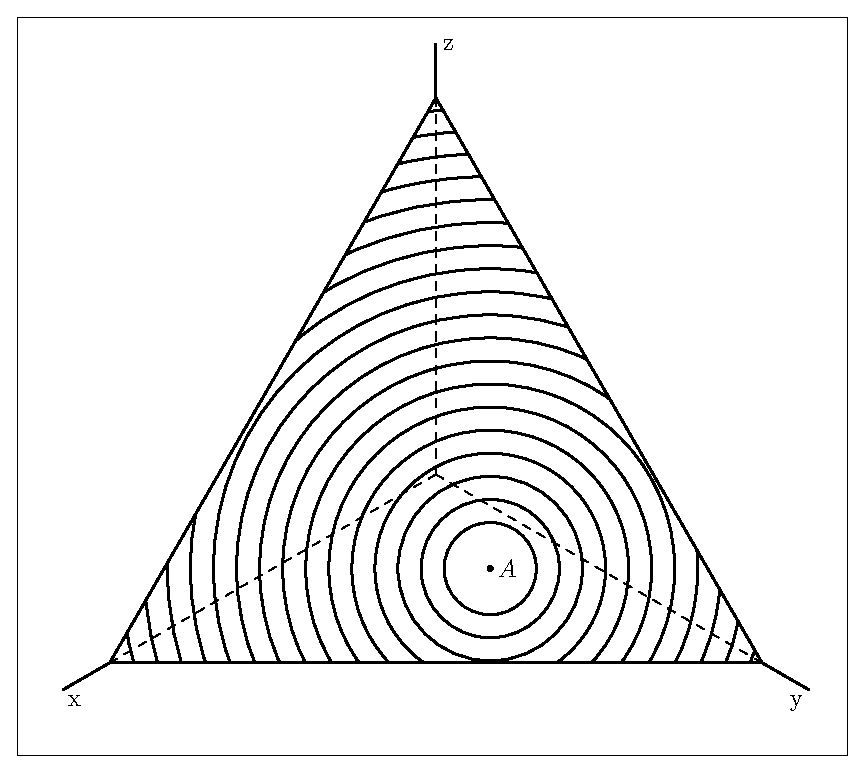
\includegraphics[width=\textwidth]{contourslp.eps}
      \caption{\footnotesize The simplex $\mathbb{S}^{2}$ in
        three-dimensional space $\mathbb{R}^{3}$ with contour lines
        corresponding to the geometry of reason around point $A$ in
        equation (\ref{eq:e6}). Points on the same contour line are
        equidistant from $A$ with respect to the Euclidean metric.
        Compare the contour lines here to figure
        \ref{fig:contoursrj}. Note that this diagram and all the
        following diagrams are frontal views of the simplex.}
      \label{fig:contourslp}
    \end{minipage}
  \end{flushright}
\end{figure}

\begin{figure}[ht]
  \begin{flushright}
    \begin{minipage}[h]{.7\linewidth}
      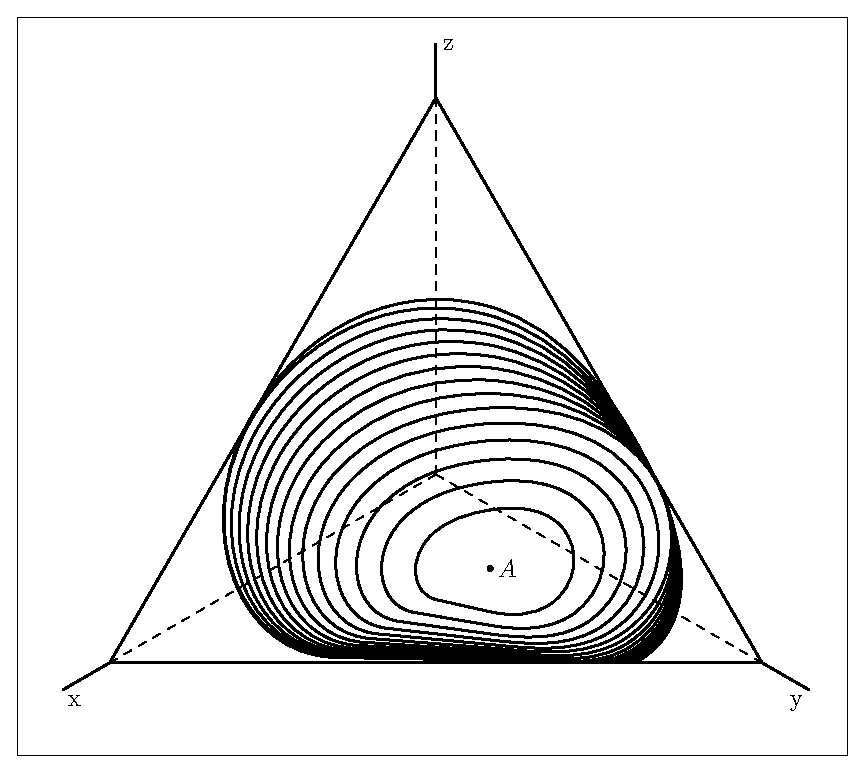
\includegraphics[width=\textwidth]{crj.eps}
      \caption{\footnotesize The simplex $\mathbb{S}^{2}$ with contour
        lines corresponding to information theory around point $A$ in
        equation (\ref{eq:e6}). Points on the same contour line are
        equidistant from $A$ with respect to the Kullback-Leibler
        divergence. The contrast to figure \ref{fig:contourslp} will
        become clear in much more detail in the body of the paper.
        Note that the contour lines of the geometry of reason are
        insensitive to the boundaries of the simplex, while the
        contour lines of information theory reflect them. One of the
        main arguments in this paper is that information theory
        respects epistemic intuitions we have about asymmetry:
        proximity to extreme beliefs with very high or very low
        probability influences the topology that is at the basis of
        updating.}
      \label{fig:contoursrj}
    \end{minipage}
  \end{flushright}
\end{figure}

\begin{figure}[ht]
  \begin{flushright}
    \begin{minipage}[h]{.7\linewidth}
      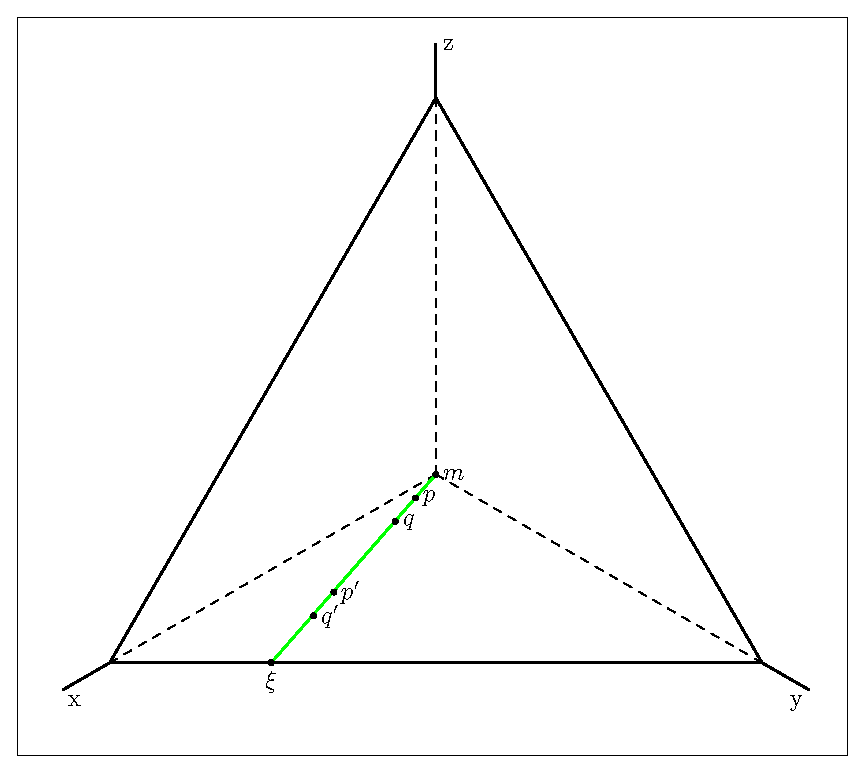
\includegraphics[width=\textwidth]{horeff.eps}
      \caption{\footnotesize An illustrations of conditions (i)--(iii)
        for \textsc{collinear horizon} in \textbf{List B}. $p,p'$ and $q,q'$
        must be equidistant and collinear with $m$ and $\xi$. If
        $q,q'$ is more peripheral than $p,p'$, then \textsc{collinear
          horizon} requires that $|d(p,p')|<|d(q,q')|$.}
      \label{fig:conditions}
    \end{minipage}
  \end{flushright}
\end{figure}

\begin{figure}[ht]
  \begin{flushright}
    \begin{minipage}[h]{.7\linewidth}
      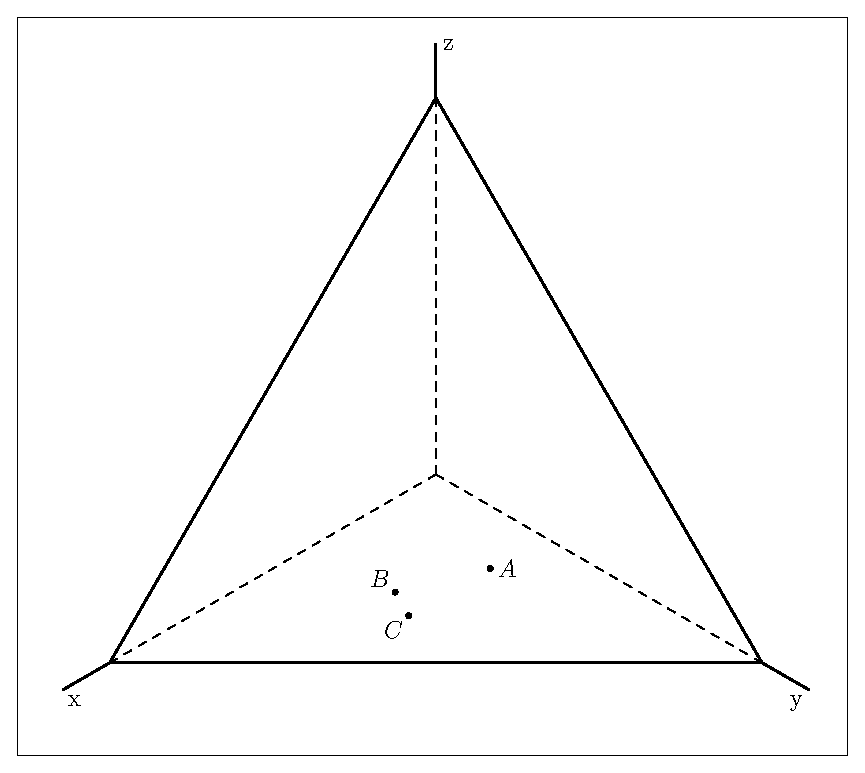
\includegraphics[width=\textwidth]{threepoints.eps}
      \caption{\footnotesize The simplex $\mathbb{S}^{2}$ in
        three-dimensional space $\mathbb{R}^{3}$ with points $a,b,c$
        as in equation (\ref{eq:e6}) representing probability
        distributions $A,B,C$. Note that geometrically speaking $C$ is
        closer to $A$ than $B$ is. Using the Kullback-Leibler
        divergence, however, $B$ is closer to $A$ than $C$ is.}
      \label{fig:threepoints}
    \end{minipage}
  \end{flushright}
\end{figure}

\begin{figure}[ht]
    \begin{minipage}[h]{.7\linewidth}
      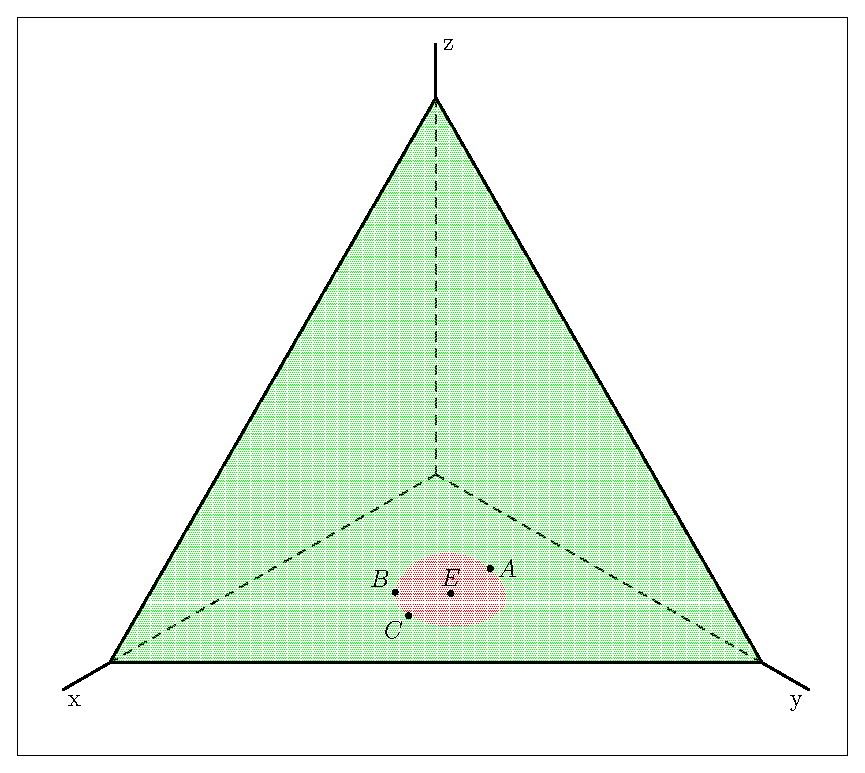
\includegraphics[width=\textwidth]{dreieck.eps}
      \caption{The zero-sum line between $A$ and $C$ is the boundary
        line between the green area, where the triangle inequality
        holds, and the red area, where the triangle inequality is
        violated. The posterior probability distribution $B$
        recommended by Jeffrey conditioning always lies on the
        zero-sum line between the prior $A$ and the LP posterior $C$,
        as per equation (\ref{eq:ocidocho}). $E$ is the point in the
        red area where the triangle inequality is most efficiently
        violated. Even though it can be calculated using the Lambert W
        function,
        $e_{k}=\frac{c_{k}}{W\left(\frac{c_{k}}{a_{k}}\exp(1+\lambda)\right)}$,
        with $\lambda$ chosen to fulfill $\sum{}e_{k}=1$, it is not
        clear to me whether $E$ is the midpoint between $A$ and $C$ or
        not.}
      \label{fig:eugoohue}
\end{minipage}
\end{figure}

\begin{figure}[ht]
  \begin{flushright}
    \begin{minipage}[h]{\linewidth}
     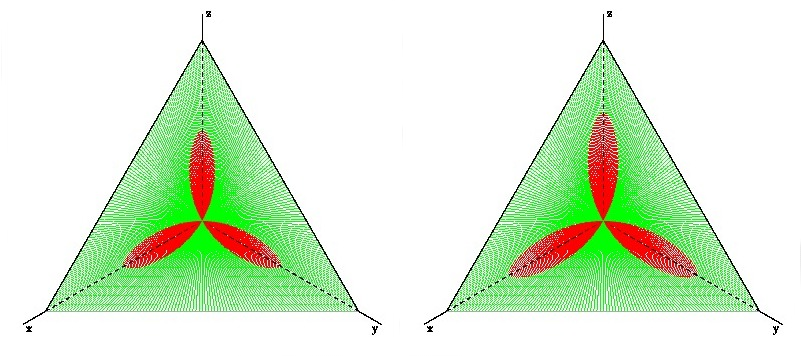
\includegraphics[width=\textwidth]{fleur-concat-edited.png}
      \caption{\footnotesize These two diagrams illustrate
        inequalities (\ref{eq:iengaech}) and (\ref{eq:feovaivo}). The
        former displays all points in red which violate
        \textsc{collinear horizon}, measured from the centre. The
        latter displays points in different colours whose orientation
        of asymmetry differs, measured from the centre. The two red
        sets are not the same, but there appears to be a relationship,
        one that ultimately I suspect to be due to the more basic
        property of asymmetry.}
      \label{fig:eeghoomo}
    \end{minipage}
  \end{flushright}
\end{figure}

\begin{figure}[ht]
  \begin{flushright}
    \begin{minipage}[h]{\linewidth}
      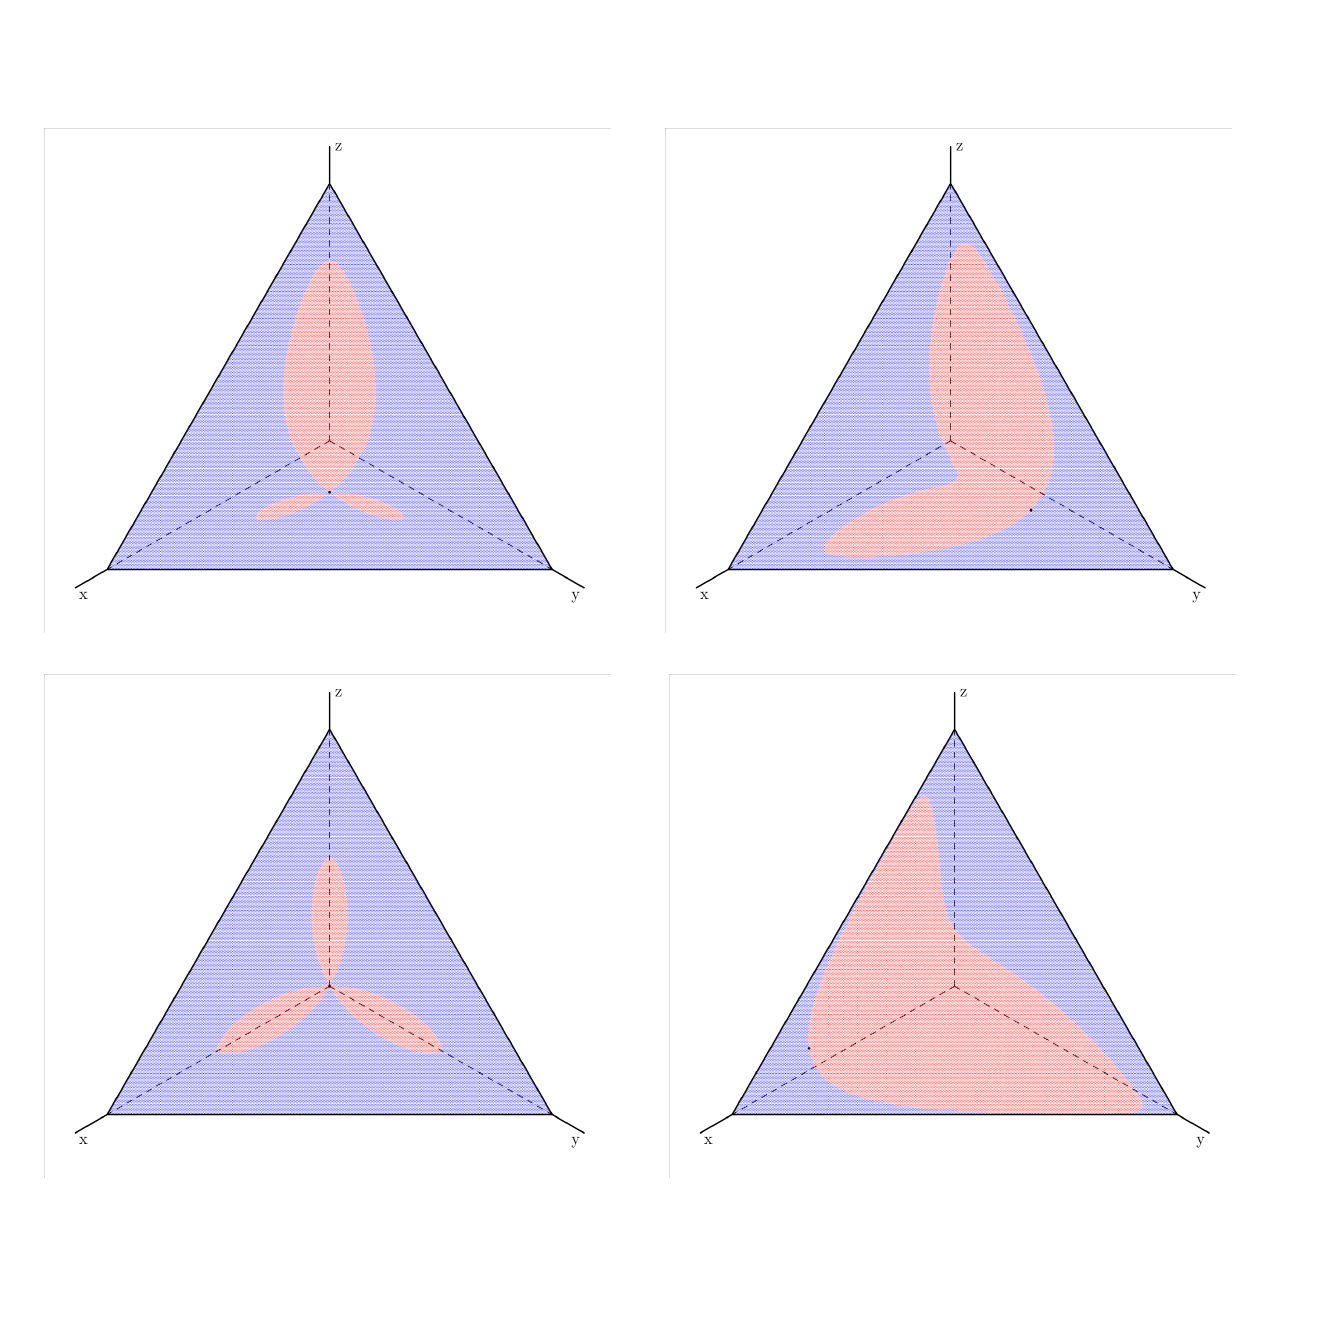
\includegraphics[width=\textwidth]{concat2.png}
      \caption{\footnotesize The partition (\ref{eq:sieruxis}) based
        on different values for $P$. From top left to bottom right,
        $P=(0.4,0.4,0.2); P=(0.242,0.604,0.154); P=(1/3,1/3,1/3);
        P=(0.741,0.087,0.172)$.
        Note that for the geometry of reason, the diagrams are
        trivial. The challenge for information theory is to explain
        the non-triviality of these diagrams epistemically without
        begging the question.}
      \label{fig:concat}
    \end{minipage}
  \end{flushright}
\end{figure}

\subsection{Transitivity of Asymmetry}
\label{subsec:Asymmetry}

Asymmetry presents a problem for the geometry of reason as well as for
information theory. For the geometry of reason, the problem is akin to
\textsc{continuity}. For information theory, the problem is the
non-trivial nature of the asymmetries it induces, which somehow need
to be reconnected to epistemic justification. I will consider this
problem in a moment, but first I will have a look at the problem for
the geometry of reason.

Extreme probabilities are special and create asymmetries in updating:
moving in direction from certainty to uncertainty is asymmetrical to
moving in direction from uncertainty to certainty. Geometry of
reason's metric topology, however, allows for no asymmetries.

\begin{quotex}
  \beispiel{Extreme Asymmetry}\label{ex:extreme} Consider two cases
  where for case 1 the prior probabilities are $Y_{1}=(0.4,0.3,0.3)$
  and the posterior probabilities are $Y_{1}'=(0,0.5,0.5)$; for case 2
  the prior probabilities are reversed, so $Y_{2}=(0,0.5,0.5)$ and the
  posterior probabilities $Y_{2}'=(0.4,0.3,0.3)$.
\end{quotex}

Case 1 is a straightforward application of standard conditioning. Case
2 is more complicated: what does it take to raise a prior probability
of zero to a positive number? In terms of information theory, the
information required is infinite. Case 2 is also not compatible with
standard conditioning (at least not with what Alan H{\'a}jek calls the
ratio analysis of conditional probability, see \scite{7}{hajek03}{}).
The geometry of reason may want to solve this problem by signing on to
a version of regularity, but then it violates \textsc{regularity}.
Happy kids, clean house, sanity: the hapless homemaker must pick two.
The third remains elusive. Continuity, a consistent view of
regularity, and symmetry: the hapless geometer of reason cannot have
it all.

Now turn to information theory. Given the asymmetric similarity
measure of probability distributions that information theory requires
(the Kullback-Leibler divergence), a prior probability distribution
$P$ may be closer to a posterior probability distribution $Q$ than $Q$
is to $P$ if their roles (prior-posterior) are reversed. That is just
what we would expect. The problem is that there is another posterior
probability distribution $R$ where the situation is just the opposite:
prior $P$ is further away from posterior $R$ than prior $R$ is from
posterior $P$. And whether a probability distribution different from
$P$ is of the $Q$-type or of the $R$-type escapes any epistemic
intuition.

For simplicity, let us consider probability distributions and their
associated credence functions on an event space with three mutually
exclusive and jointly comprehensive atoms
$\Omega=\{\omega_{1},\omega_{2},\omega_{3}\}$. The simplex
$\mathbb{S}^{2}$ represents all of these probability distributions.
Every point $p$ in $\mathbb{S}^{2}$ representing a probability
distribution $P$ induces a partition on $\mathbb{S}^{2}$ into points
that are symmetric to $p$, positively skew-symmetric to $p$, and
negatively skew-symmetric to $p$ given the topology of information
theory.

In other words, if

\begin{equation}
  \label{eq:sksy}
  \Delta_{P}(P')=D_{\mbox{\tiny KL}}(P',P)-D_{\mbox{\tiny KL}}(P,P'),
\end{equation}

then, holding $P$ fixed, $\mathbb{S}^{2}$ is partitioned into three
regions, 

\begin{equation}
  \label{eq:sieruxis}
  \Delta^{-1}(\mathbb{R}_{>0})\hspace{.5in}\Delta^{-1}(\mathbb{R}_{<0})\hspace{.5in}\Delta^{-1}(\{0\})
\end{equation}

One could have a simple epistemic intuition such as \qnull{it takes
  less to update from a more uncertain probability distribution to a
  more certain probability distribution than the reverse direction,}
where the degree of certainty in a probability distribution is
measured by its entropy. This simple intuition accords with what we
said about extreme probabilities and it holds true for the asymmetric
distance measure defined by the Kullback-Leibler divergence in the
two-dimensional case where $\Omega$ has only two elements.

In higher-dimensional cases, however, the tripartite partition
(\ref{eq:sieruxis}) is non-trivial---some probability distributions
are of the $Q$-type, some are of the $R$-type, and it is difficult to
think of an epistemic distinction between them that does not already
presuppose information theory (see figure~\ref{fig:concat} for
illustration).

On any account of well-behaved and ill-behaved asymmetries, the
Kullback-Leibler divergence is ill-behaved. Of the four axioms as
listed by Ralph Kopperman for a distance measure $d$ (see
\scite{8}{kopperman88}{89}), the Kullback-Leibler divergence violates
both symmetry and triangularity, making it a \qnull{semi-quasimetric}:

\begin{enumerate}[(m1)]
\item $d(x,x)=0$ (self-similarity)
\item $d(x,z)\leq{}d(x,y)+d(y,z)$ (triangularity)
\item $d(x,y)=d(y,x)$ (symmetry)
\item $d(x,y)=0$ implies $x=y$ (separation)
\end{enumerate}

The Kullback-Leibler divergence not only violates symmetry and
triangularity, but also \textsc{transitivity of asymmetry}. For a
description of \textsc{transitivity of asymmetry} see \textbf{List B}.
For an example of it, consider

\begin{equation}
  \label{eq:transviol}
    P_{1}=\left(\frac{1}{2},\frac{1}{4},\frac{1}{4}\right)  \hspace{.5in}
    P_{2}=\left(\frac{1}{3},\frac{1}{3},\frac{1}{3}\right) \hspace{.5in}
    P_{3}=\left(\frac{2}{5},\frac{2}{5},\frac{1}{5}\right)
\end{equation}

In the terminology of \textsc{transitivity of asymmetry} in \textbf{List B},
$(P_{1},P_{2})$ is asymmetrically positive, and so is $(P_{2},P_{3})$.
The reasonable expectation is that $(P_{1},P_{3})$ is asymmetrically
positive by transitivity, but for the example in (\ref{eq:transviol})
it is asymmetrically negative.

How counterintuitive this is (epistemically and otherwise) is
demonstrated by the fact that in MDS (the multi-dimensional scaling of
distance relationships) almost all asymmetric distance relationships
under consideration are asymmetrically transitive in this sense, for
examples see international trade in \scite{7}{chino78}{}; journal
citation in \scite{7}{coombs64}{}; car switch in
\scite{7}{harshmanetal82}{}; telephone calls in
\scite{7}{harshmanlundy84}{}; interaction or input-output flow in
migration, economic activity, and social mobility in
\scite{7}{coxonetal82}{}; flight time between two cities in
\scite{8}{gentleman06}{191}; mutual intelligibility between Swedish
and Danish in \scite{8}{vanommenetal13}{193}; Tobler's wind model in
\scite{7}{tobler75}{}; and the cyclist lovingly hand-sketched in
\scite{8}{kopperman88}{91}.

This \qnull{ill behaviour} of information theory begs for explanation,
or at least classification (it would help, for example, to know that
all reasonable non-commutative difference measures used for updating
are ill-behaved). For a future research project, it would be
interesting either to see information theory debunked in favour of an
alternative geometry (this paper has demonstrated that this
alternative will not be the geometry of reason); or to see uniqueness
results for the Kullback-Leibler divergence to show that despite its
ill behaviour the Kullback-Leibler is the right asymmetric distance
measure on which to base inference and updating.

\newpage

% BibTeX users please use one of
\bibliographystyle{spbasic}      % basic style, author-year citations
%\bibliographystyle{spmpsci}      % mathematics and physical sciences
%\bibliographystyle{spphys}       % APS-like style for physics
\bibliography{bib-2902}

% Non-BibTeX users please use
% \begin{thebibliography}{}
%
% and use \bibitem to create references. Consult the Instructions
% for authors for reference list style.
%
% \bibitem{RefJ}
% Format for Journal Reference
% Author, Article title, Journal, Volume, page numbers (year)
% Format for books
% \bibitem{RefB}
% Author, Book title, page numbers. Publisher, place (year)
% etc
% \end{thebibliography}

\end{document}
% end of file template.tex

